\chapter{Методы извлечения и сравнения уникальных особенностей радужки}
\label{chapter:fem_methods}

Завершающими и неотъемлемыми частями алгоритма распознавания являются: извлечение уникальных особенностей (признаков) биометрического образца (-ов) и его (их) последующего сравнения, по результатам которого вычисляется степень схожести, используемая для принятия решения. Оба этапа обычно рассматриваются в едином контексте, т.к. являются смежными и сильно зависят друг от друга.

Извлекаемые признаки должны обладать следующими общими свойствами~\cite{jain_2004,matveev_doctor_thesis}:

\begin{enumerate}
	\item[$\bullet$] Уникальность (информативность/значимость): признаки должны содержать в себе информацию, достаточную для того, чтобы обеспечить отличаемость биометрического образца от других;
	\item[$\bullet$] Стабильность (устойчивость): неизменность во времени, независимость от условий регистрации и изменчивости самого образца;
	\item[$\bullet$] Применимость: признаки должны быть легко извлекаемыми, сравниваемыми и храниться в компактном виде.
\end{enumerate}

С точки зрения анатомии, для радужки можно выделить несколько основных источников для извлечения признаков: цвет радужки, форма зрачка, текстура радужки и др. Самыми информативным признаками радужки являются характеристики её текстуры~\cite{daugman_how_works}. Процедуре извлечения особенностей текстуры обычно предшествует этап нормализации (нормирования) изображения, представляющая собой конформное кольца радужки в прямоугольник, называемое полярным преобразованием (\ref{eq:certesian-polar}). Из литературы известно несколько вариантов такого преобразования, описанных в работе~\cite{arvacheh_2006}.

Обзоры различных методов извлечения и сравнения особенностей радужки приведены в работах~\cite{bowyer_survey_2008, bowyer_handbook_2012, ng_overview_2008, rathgeb_2011}. Среди модификаций можно выделить базовые подходы~\cite{matveev_doctor_thesis}: использование двумерных вейвлетов Габора~\cite{daugman_how_works}, использование матриц совместной встречаемости~\cite{gupta_2005,zaim_2006}, использование расположения и хаарктеристик ключевых точек текстуры~\cite{pranith_2010}, применение дискретного косинусного преобразования~\cite{monro_2007}, использование одномерный вейвлетов различных масштабов~\cite{boles_1998}, различные варианты преобразования Хаара~\cite{lim_2001,popescu_2011}, пирамиды Лапласа~\cite{wildes_1994}, метод основанный на ориентации градиентов~\cite{takano_2011}. В большинстве недавних работ предлагается использование методов глубокого обучения~\cite{liu_2016_di,gangwar_2016,proenca_2017,zhao_2017,tang_2017}.

Специфика использования мобильного устройства (\ref{sec:main_difficulties_mobile},~\ref{sec:mobile_iris_features}) сказывается на качестве выделения области радужки (\ref{sec:hard_condition_segm_features}) и изменчивости текстуры радужки (\ref{sec:iris-structure-and-properties},~\ref{sec:auth_method}). Следствием этих факторов является высокая вариативность входных данных для методов извлечения и сравнения этих особенностей. Это ограничивает возможности алгоритмов извлечения признаков, вызывая значительные внутриклассовые отклонения.

\section{Вейвлеты Габора и адаптивное квантование фазы}
\label{sec:gabor-and-quantization}

Одним из наиболее распространенных подходов извлечения особенностей и представления их в виде некоторого вектора признаков (т.н. эталона) радужки является использование вейвлетов Габора. В качестве входной информации используется нормализованное изображение радужки и бинарная маска, описывающая полезную и зашумленную (ресницы, веки, блики и др.) области изображения. Базовая структура такого подхода изображена на Рис.~\ref{fig:irec-basic-stages-gabor}.

\begin{figure}[ht!]
	\begin{center}
		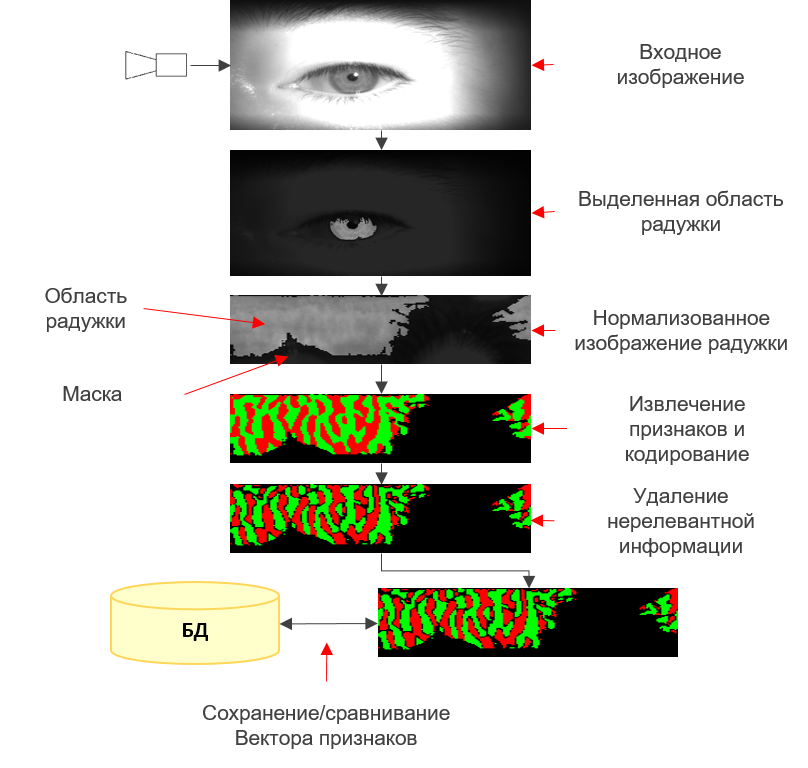
\includegraphics[width=0.75\columnwidth]{pictures/irec-basic-stages-gabor.png}
		\caption{Общая схема алгоритма извлечения и сравнения признаков радужки при помощи вейвлетов Габора}
		\label{fig:irec-basic-stages-gabor}
	\end{center}
\end{figure}

Методы, основанные на применении вейвлетов Габора, являются одними из самых распространенных для не мобильных приложений, т.к. способны обеспечивать достаточную точность и надежность~\cite{daugman_how_works}. Процедура кодирования, присущая таким методам (Рис.~\ref{fig:fem-filter-and-quant}), необходима, в частности, для повышения стабильности представления вектора признаков и ускорения процесса сравнения. Одним из наиболее распространенных подходов к кодированию является бинарное квантование значений вектора признаков. Несмотря на то что квантование способно не учитывать нерелевантную, оно также способствует уменьшению полезной информации, дестабилизируя тем самым значения вектора признаков~\cite{hollingsworth_2009,proencca_2015}. Метод по-прежнему имеет одно важное преимущество, сделавшее его настолько популярным для использования: сравнение квантованных значений - битовая операция, а значит метод позволяет осуществлять сравнения с очень высокой скоростью. Эта особенность является очень важной, в частности, при решении задачи идентификации, когда требуется произвести поиск максимально похожего образца по базе данных, насчитывающей большое количество примеров.

\medspace
\begin{figure}[h]
	\begin{center}
		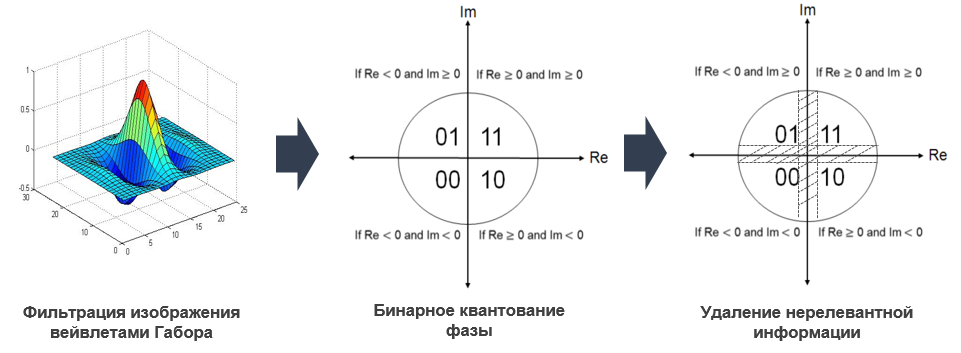
\includegraphics[width=0.95\columnwidth]{pictures/fem-filter-and-quant.png}
		\caption{Извлечение вектора признаков радужки вейвлетами Габора и последующее квантование}
		\label{fig:fem-filter-and-quant}
	\end{center}
\end{figure}

\noindent
Современные модификации подхода рассматривают понятие хрупкости как неустойчивость элементов вектора без учета характера появления такой неустойчивости. В работе предлагается разделение источников нестабильности на естественные и вызванные кодированием. Предлагается новый подход к построению вектора признаков радужной оболочки. Подход состоит из двух этапов: извлечения первичных признаков с использованием фильтрации единичным вейвлетом Габора, параметра которого заранее оптимизированы, и адаптивного квантованием с предварительно оптимизированными порогами хрупкости.

\subsection{Извлечение вектора признаков}
\label{sec:fe-gabor}

Один из методов извлечения признаков, используемый во многих успешных коммерческих системах распознавания по радужке, основан на извлечении квантованных значений фазы после свертки нормализованного изображения с набором комплексных фильтров Габора. Этот метод был впервые предложен в работе~\cite{daugman_1993} и с тех пор подвергался различным модификациям~\cite {si_2012, thornton_2007}. Все связанные подходы используют либо несколько фильтров с октавным увеличением частоты, либо с одним фильтром с заранее заданными параметрами. Основным преимуществом метода Габора, применяемого в этом случае, является его способность создавать полосовой фильтр с регулируемыми параметрами. Это свойство позволяет учесть априорные характеристики анализируемого объекта в частотной области. В неидеальных условиях с наличием коррелированного шума, вызванного низкочастотной разницей яркости, можно добиться более высокого качества распознавания при настройке тонкого полосового фильтра путем оптимизации его параметров.

\medspace
\begin{figure}[h]
	\begin{center}
		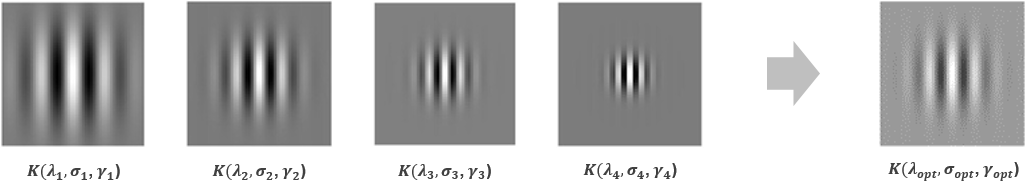
\includegraphics[width=0.95\columnwidth]{pictures/gabor-kernels.png}
		\caption{Переход от использования нескольких ядер к одному с оптимальными параметрами}
		\label{fig:gabor-kernels}
	\end{center}
\end{figure}

Предложен подход, использующий один фильтр с заранее оптимизированными параметрами (Рис.~\ref{fig:gabor-kernels}), различными для действительной $Re$ и мнимой $Im$ частей. Для оптимизации были выбраны следующие параметры ядра: длина волны $\lambda$, стандартное отклонение $\sigma$ и пространственное соотношение сторон $\gamma$ соответственно. Многие эксперименты, проведенные нами и другими исследователями, показали, что наиболее значимые черты радужки ортогональны ее радиальному направлению, поэтому устанавливается $\theta=0$. В качестве целевой функции для оптимизации выбрано значение $EER$, отражающее частоту ошибок, соответствующую пороговому значению $t$, для которого $FMR$ равна $FNMR$: $FMR(t)=FNMR(t)$. Выбор $EER$ в качестве целевой функции позволяет оценить эффективность системы распознавания независимо от заранее определенного порога для степени схожести. Для оптимизации использовался метод прямого поиска Нелдера-Мида~\cite{nelder_mead_1965}. Этот метод хорошо зарекомендовал себя при решении задач оптимизации, в частности, в случае наличия областей плато и седловых точек из-за его способности к нерегулярной конструкции симплекса. Оптимизация и окончательное тестирование выполнялись на наборе данных CASIA-IrisV3-Lamp~\cite{casia_v3_lamp}, симулирующем изменение освещенности в процессе регистрации изображения. Весь набор данных был разделен для обучающую и тестовую выборки в пропорции 0.6/0.4.

\begin{table}[h]
\centering
	\begin{tabular}{|l|c|c|}\hline
		\textbf{Метод}						&\textbf{EER}	&\textbf{d'}\\\hline
		OFI~\cite{daugman_1993}		&0.0406	&3.61\\
		Предложенный метод			&0.0373	&3.73\\
		\hline
	\end{tabular}
	\caption{Результаты по точности распознавания для двух алгоритмов извлечения особенностей радужки вейвлетам Габора при фиксированном алгоритме квантования}
	\label{tab:gabor_eer}
\end{table}

Сравнение метода производилось с базовым подходом с октавным увеличением частоты ядра (octave frequency increase, OFE), описанным в  работе~\cite{daugman_1993}. С целью демонстрации преимуществ обоих частей (фильтрации и квантования) предложенного метода, в качестве первого эксперимента было произведено сравнение методов фильтрации для фиксированного метода квантования. Расстояние Хэмминга (Hamming Distance, HD) выбирана в качестве меры различия пар векторов признаков радужки. Результаты представлены в таблице~\ref{tab:gabor_eer}. Для оценки, кроме значения $EER$, была так еж использована метрика $d'$, отражающая степень разделимости между полученными распределениями genuine (своих) и impostor (самозванцев). Данный показатель оказывается более чувствительным и информативным, когда выполняются условия: распределения имеют не большую площадь пересечения, распределения имеют вид Гауссового.

Результаты эксперимента (Таб.~\ref{tab:gabor_eer}) отражают преимущества предложенного подхода. Стоит также отметить, что предлагаемый метод требует двух операций свертки (по одному для частей $Re$ и $Im$ соответственно), тогда как для OFI-метода требуется по крайней мере четыре (Рис.~\ref{fig:gabor-kernels}) для каждой части (всего восемь). Т.к. размер ядра для свертки для обоих методов был выбран идентичным, можно заключить, что предложенный метод в 4 раза превосходит OFI по скорости.

\subsection{Квантование}
\label{sec:quantization}

Квантование фазы, полученного после фильтрации сигнала, является заключительным этапом процедуры построения вектора признаков (Рис.~\ref{fig:irec-basic-stages-gabor}). В оригинальной работе квантование производится в зависимости от знака фазы~\cite{daugman_1993}, и все элементы используются для сравнения. Кроме того, в работе~\cite{hollingsworth_2009} было показано, что не все квантованные элементы вектора признаков одинаково важны и вводится понятие хрупкости. Хрупкость в данном конкретном случае означает несогласованность информации, хранящейся в двух или более векторах одной и той же радужки. Несогласованные элементы могут быть определены из нескольких или из одного кадра. Данная работа ориентирована на однокадровый подход. Большинство современных работ~\cite{lee_2013,hollingsworth_2009} используют константное предопределенное пороговое значение (одинаковое для $Re$ и $Im$) для классификации векторных элементов на хрупкие и не-хрупкие.

\begin{figure}[h]
	\begin{center}
		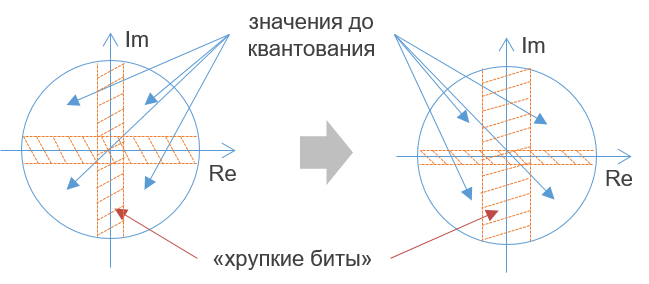
\includegraphics[width=0.75\columnwidth]{pictures/re_im_different_ths.png}
		\caption{Задание значений порогов различных для $Re$ and $Im$ частей}
		\label{fig:re_im_different_ths}
	\end{center}
\end{figure}

Предложенный метод подразумевает задание различных и независимых друг от друга порогов для $Re$ and $Im$ частей(Рис.~\ref{fig:re_im_different_ths}).

\begin{figure}[ht!]
	\begin{center}
		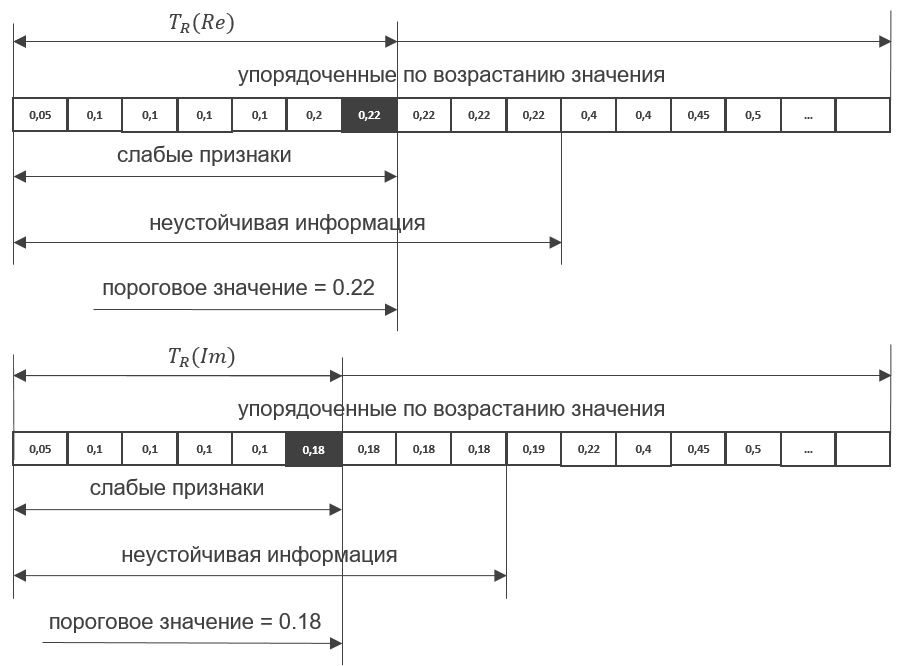
\includegraphics[width=0.95\columnwidth]{pictures/thresh_determination.png}
		\caption{Определение порога хрупкости}
		\label{fig:thresh_determination}
	\end{center}
\end{figure}

Алгоритм адаптивного определения порога хрупкости использует опорное значение $T_R$, полученное после оптимизации и состоит из следующих этапов:

\begin{enumerate}
	\setlength\itemsep{0em}\setlength\parskip{0em}\setlength\topsep{0em}\setlength\partopsep{0em}\setlength\parsep{0em} 
	\item{Значения вектора признаков упорядочиваются по возрастанию $FV=\left\lbrace min..max \right\rbrace $}
	\item{Финальное значение порога хрупкости определяется как $T_F=FV[T_R*L]$, где $L$ размерность вектора признаков (Рис.~\ref{fig:thresh_determination})}
\end{enumerate}

Опорные значения порогов $T_R(Re)$ и $T_R(Im)$ получены по результатам предварительной оптимизации на обучающей выборке полным перебором. Полученные значения $T_F(Re)$ и $T_F(Im)$ используются далее для удаления неустойчивой информации из вектора признаков после квантования.

{\bf Описание базы данных}
\label{sec:fem-gabor-dataset-desc}

Предложенный метод извлечение признаков проверяется на двух разных базах данных изображений радужек, полученных при помощи цифровой камеры в БИК диапазоне. Один из них CASIA-IrisV3-Lamp~\cite{casia_v3_lamp} является общедоступным и содержит изображения, снятые в условиях изменяющегося уровня освещенности (примеры изображений на Рис.~\ref{fig:fem-gabor-db-examples-casiav3}). Другой набор данных был собран приватно при помощи мобильного устройства, но в сильно меняющихся условиях окружающей среды: в помещении при нормальном освещении, в темном помещении и на ярком солнце, симулируя попытки аутентификации. Описание собранной БД приведено в таблице~\ref{tab:fem-gabor-dataset-spec}, а примеры изображений приведены на Рис.~\ref{fig:fem-gabor-db-examples-mobile}. Параметры фильтра Габора, а также пороговые значения хрупкости ($T_R$) предварительно оптимизированы для каждого набора данных независимо друг от друга.

\medspace
\begin{figure}[h]
	\begin{center}
		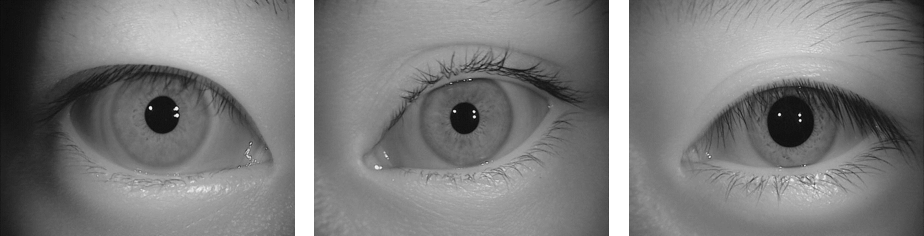
\includegraphics[width=0.75\columnwidth]{pictures/fem-gabor-db-examples-casiav3.png}
		\caption{Примеры изображений радужек из набора данных CASIA-IrisV3-Lamp}
		\label{fig:fem-gabor-db-examples-casiav3}
	\end{center}
\end{figure}

\begin{figure}[h]
	\begin{center}
		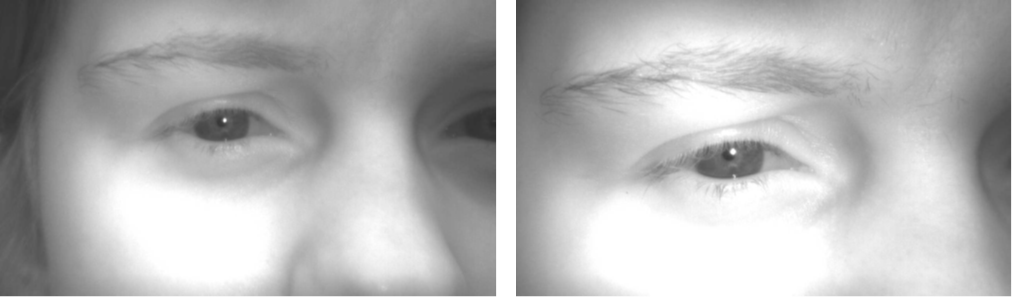
\includegraphics[width=0.75\columnwidth]{pictures/fem-gabor-db-examples-mobile.png}
		\caption{Примеры изображений радужек из набора данных, собранных при помощи мобильного устройства}
		\label{fig:fem-gabor-db-examples-mobile}
	\end{center}
\end{figure}

\begin{table}[h]
	\centering
	\begin{tabular}{|l|c|c|} \hline
		\textbf{Набор данных}					& \textbf{CASIA-IrisV3-Lamp}		& \textbf{Мобильный}\\\hline
		Кол-во субъектов 				& $411$					& $286$\\					
		Кол-во классов 					& $819$					& $566$\\
		Расы 							& $Азиаты$				& $Азиаты и Европеоиды$\\
		Кол-во радужек на изображении 	& $1$					& $1$\\
		Дистанция съемки 				& $15\div25$ (см)		& $15\div35 (см)$\\
		Разрешение камеры (пикс.) 		& $640\times480$		& $1280\times720$\\
		\hline
	\end{tabular}
	\caption{Описание баз данны тестирования}
	\label{tab:fem-gabor-dataset-spec}
\end{table}

{\bf Экспериментальные результаты}
\label{sec:fem-gabor-exp-results}

Оценивание предложенного метода адаптивного квантования производилось по значениям $ERR$ и $d'$. В качестве метода для сравнения была взята работа~\cite{hollingsworth_2009}. Предложенный и описанный выше метод извлечения признаков при помощи фильтра Габора был использован в качестве основанного для извлечения признаков для обоих методов. Результаты представлены в Таб.~\ref{tab:fem-gabor-quant-exp-results}.

\begin{table}[h]
	\centering
	\begin{tabular}{|l|c|c|c|c|}\hline
		\textbf{Dataset}&\multicolumn{2}{c|}{\textbf{CASIA-IrisV3-Lamp}}&\multicolumn{2}{c|}{\textbf{Мобильный}}\\\hline
												&EER		&d'			&EER		&d'\\
		Без квантования							&0.0373		&3.73		&0.0048		&7.62\\
		Hollingsworth~\cite{hollingsworth_2009}	&0.0430		&3.60		&0.0043		&7.77\\
		Предложенный							&0.0370		&3.85		&0.0040		&8.01\\
		\hline
	\end{tabular}
	\caption{Результаты сравнения методов квантования}
	\label{tab:fem-gabor-quant-exp-results}
\end{table}

Результаты эксперимента демонстрируют превосходство метода по сравнению с~\cite{hollingsworth_2009} на обоих наборах данных.

\section{Метод с использованием глубокого обучения}
\label{sec:fem-deep}

Относительно новым и одним из наиболее перспективных направлений в области биометрического распознавания, как и во многих других областях, является применение методов глубокого обучения. О преимуществах и недостатках подходов, построенных на глубоком обучении, упоминалось ранее (\ref{sec:segm_existing_app_overview}). Первые работы, использующие такой подход в применении к задаче извлечения и сравнения уникальных особенностей радужной оболочки глаза начали появляться в 2016 году. Отправной точкой была работа Liu и др.~\cite{liu_2016_di}, названная DeepIris. Чуть позже Minae и др. в работе~\cite{minaee_2016} провели анализ применимости подхода с извлечением признаков радужки при помощи нейронной сети, предварительно обученной на базе данных изображений ImageNet, содержащей порядка тысячи классов различных объектов. В качестве вектора признаков в таком подходе выступает вектор выходных значений, т.н. эмбеддингов (embedings), последнего полносвязного слоя сети. В работе предложено использовать данный вектор без какого-либо дополнительного обучения и подстройки параметров сети. Далее метод главных компонент (PCA) используется для понижения размерности вектора и метод опорных векторов (SVM) для классификации на genuine и impostor. В качестве базовой была использована архитектура VGG. Данную работу можно рассматривать как одну из первых попыток изучить возможности глубоких нейронных сетей в применении к задаче распознавания по радужной оболочке. Позднее Gangwar и др.~\cite{gangwar_2016} представили DeepIrisNet модель, объединяющую в себе перспективные методы глубокого обучения, известные на тот момент. Год спустя Tang и др.~\cite{tang_2017} представили похожу на DeepIrisNet работу, основанную на использовании эмбеддингов. В то же время Proenca и др.~\cite{proenca_2017} представили метод, который они назвали IRINA. Идея работы заключалась в том, чтобы при помощи сети осуществлять поиск соответствующих патчей для пар изображений, а также Марковские случайные поля (MRF) для компенсации нелинейных искажений текстуры радужки. В качестве классификатора было предложено использовать SVM. В работе продемонстрирована высокая устойчивость к текстурным деформациям зрачка, радужки, а также к ошибкам сегментации. Однако, предлагаемая модель существенно ограничивает применимость метода для мобильных приложений в виду собственной вычислительной сложности. Подход с парой т.н. полносверточных сетей (FCN) с модифицированной расширенной триплетной функцией потерь ETL (extended triplet loss) был предложен в работе~\cite{zhao_2017}. Одна из сетей используется для извлечения признаков радужки, а вторая осуществляет построение маски. Метод нечеткого улучшения изображения в сочетании с линейной итеративной кластеризацией и нейронной сетью SOM был предложено в~\cite{abate_2017}. Несмотря на то, что метод заявлен для распознавания на мобильном устройстве, производительность в режиме реального времени не была достигнута.

Для сравнения с предложенным подходом среди вышеперечисленных были выбраны те, которые удовлетворяют следующим критериям:

\begin{enumerate}
	\item[$\bullet$] Применимость к мобильным устройствам (способность осуществлять обработку в режиме реального времени);
	\item[$\bullet$] Высокая точность распознавания.
\end{enumerate}

Предложенный метод представляет собой сверточную нейронную сеть, спроектированную с учетом преимуществ нормализованного изображения радужки как инварианта, представления низко- и высокоуровневых признаков сравнения, а также информации об окружении. Модель состоит из двух основных частей: выделения особенностей и их последующего сравнения. Обе части обучаются совместно.

\begin{figure}[t!]
	\begin{center}
		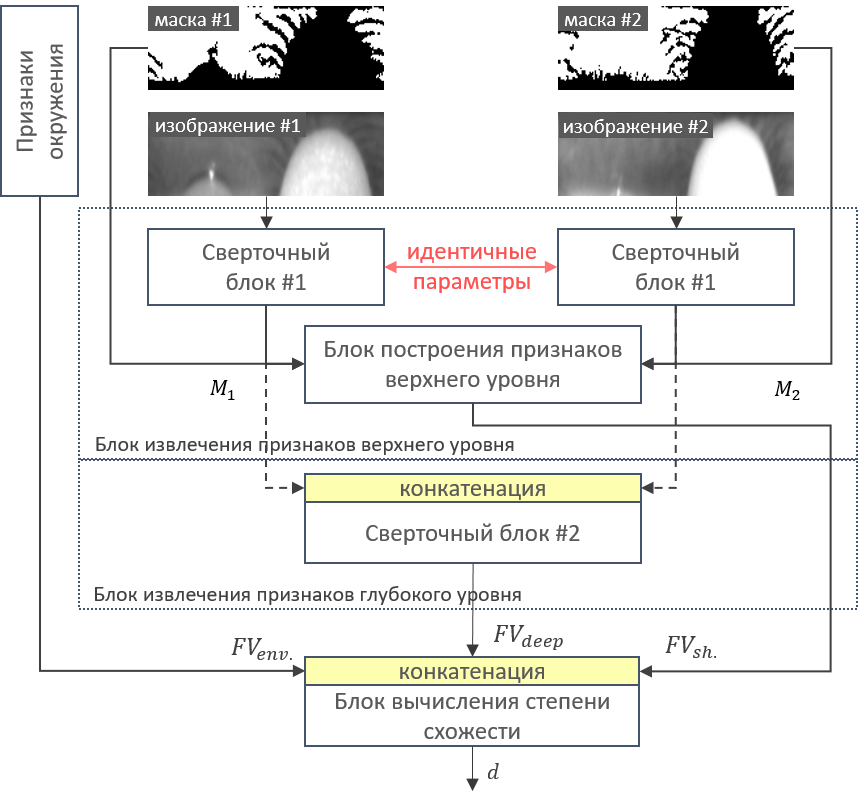
\includegraphics[width=.75\linewidth]{pictures/block-scheme-matcher.png}
	\end{center}
	\caption{Архитектура предложенной модели сверточной сети для извлечения и сравнения уникальных признаков радужки}
	\label{fig:block-scheme-matcher}
\end{figure}

\subsection{Низкоуровневое представление признаков}
\label{sec:fem-nn-shfv}

Объединение низко и высокоуровневых признаков в нейронных сетях не является новой идеей~\cite{ergun_2016,janani_2017,gao_2018}. Известно, что первые слои в CNN отвечают за извлечение низкоуровневой текстурной информации, а представление высокого уровня достигается с глубиной~\cite{zeiler_2014,harley_2015}. Методы выделения признаков радужки, основанные на различных видах вейвлет-преобразований, упомянутых ранее (вейвлеты Габора и т.д.~\cite{daugman_how_works,odinokikh_2017_fvc}), которые в течение многих лет доминировали в этой области, - это в основном попытки использовать низкоуровневое описание текстуры. Эти методы доказали свою надежность для сценариев с практически неизменным окружением, но оказались чувствительными к ее изменениям.

Нормализованное изображение радужки представляет собой инвариант, позволяющий использовать текстурные признаки в условиях слабо изменяющейся среды, когда они остаются хорошо выровненными относительно между собой. Поэтому распознавание по радужке является хорошим примером задачи, для которой рентабельность использования низкоуровневых представлений объектов может быть исследована в контексте методов на основе CNN и сильно изменяющихся условий окружения.

В работе рассматривается влияние высокоуровневых текстурных признаков на эффективность распознавания. Взяв за основу классический подход~\cite{daugman_how_works} к вычислению степени схожести при помощи расстояния Хэмминга (Hamming Distance, HD), вектор вида $FV_{sh}=\left\lbrace{x_0..x_N}\right\rbrace$ использовался в качестве описания высокоуровневых текстурных отличительных признаков. Каждый элемент $x_i$ вектора $FV_{sh}$ вычисляется следующим образом:

\begin{equation}
\label{eq:shallow-fv}
x_i = \frac{\sum|FM^{Sq}_{1,i}-FM^{Sq}_{2,i}| \times M_c}{\sum{M_c}}
\end{equation}
где $FM^{Sq}_{k,i}$ это $i$-я карта признаков $k$-й радужки (входящей или сохраненной) после стандартизации приведением к $\mu=0$ и $\sigma=1$, бинаризованная по знаку; $M_c$ - бинарная маска, используемая для выделения шума в виде ресниц, век и различных бликов, объединенная из двух: $M_c=M_1 \times M_2$.

\begin{table}
	\begin{center}
		\begin{tabular}{|c|c|}
			\hline
			\textbf{Слой}									& \textbf{Размер входного тензора} \\
			\hline
			Сверточный 3x3 $(s'=1, act.=tanh)$				& $1\times49\times161$\\
			Сверточный блок $CNNB_{MN} (k_h=k_w=3,s'=2)$ 	& $8\times47\times159$\\
			\hline
		\end{tabular}
		\caption{Структура сверточного блока \#1}
		\label{tab:conv-block-1}
	\end{center}
\end{table}

\begin{table}[h]
	\begin{center}
		\begin{tabular}{|c|c|}
			\hline
			\textbf{Слой}					&\textbf{Шаг свертки} \\
			\hline
			Свертка по глубине ($k_h=k_w=3$) 	&	$s'$\\
			Пакетная нормализация			&	$-$\\
			ReLU							& 	$-$\\
			Свертка ($k_h=k_w=1$) 			& 	$1$\\
			Пакетная нормализация			&	$-$\\
			ReLU							& 	$-$\\
			\hline
		\end{tabular}
		\caption{Структура блока $CNNB_{MN}$}
		\label{tab:dwscblock}
	\end{center}
\end{table}

Основные элементы блока выделения высокоуровневых признаков и их взаимосвязи приведены на Рис.~\ref{fig:block-scheme-matcher}, а структура сверточного блока \#1 представлена в Таб.~\ref{tab:conv-block-1}. Структура основных блоков, впервые предложенная в работе~\cite{howard_2017} как вычислительно эффективная, была выбрана в качестве базового структурного элемента архитектуры (Таб.~\ref{tab:dwscblock}). Карты признаков $FM^{Sq}_{1, i}$ и $FM^{Sq}_{2,i}$ (\ref{eq:shallow-fv}) являются выходом первого сверточного слоя с функцией активации $tanh()$ (Таб.~\ref{tab:conv-block-1}).

Распределения элементов вектора $FV_{sh}$ для genuine и impostor сравнений, полученные в процессе обучения по окончании различных эпох на валидационной выборке, представлены на Рис.~\ref{fig:shfv-distributions-combined}. Несмотря на то, что распределения для разных фильтров для поздних эпох очень похожи, сами фильтры сильно различаются (Рис.~\ref{fig:shfv-filters-100-epoch}). Форма распределений для обоих классов напоминает Гауссиан. По этой причине для оценки степени их разделимости были выбраны значения d' и EER. Изменение значений для каждого фильтра в процессе обучения представлено на Рис.~\ref{fig:eer_dprime_epochs}. Результаты, представленные в Таб.~\ref{tab:exp-results-extreme}, показывают, что добавление $FV_{sh}$ позволяет получить несколько лучшие результаты по точности распознавания для базовой модели с ядрами 3х3 на первом сверточном слое. Также показано, что для больших ядер (9x9) разница в производительности становится более значимой (Таб.~\ref{tab:exp-results-extreme}).

\begin{figure}[t!]
	\begin{center}
		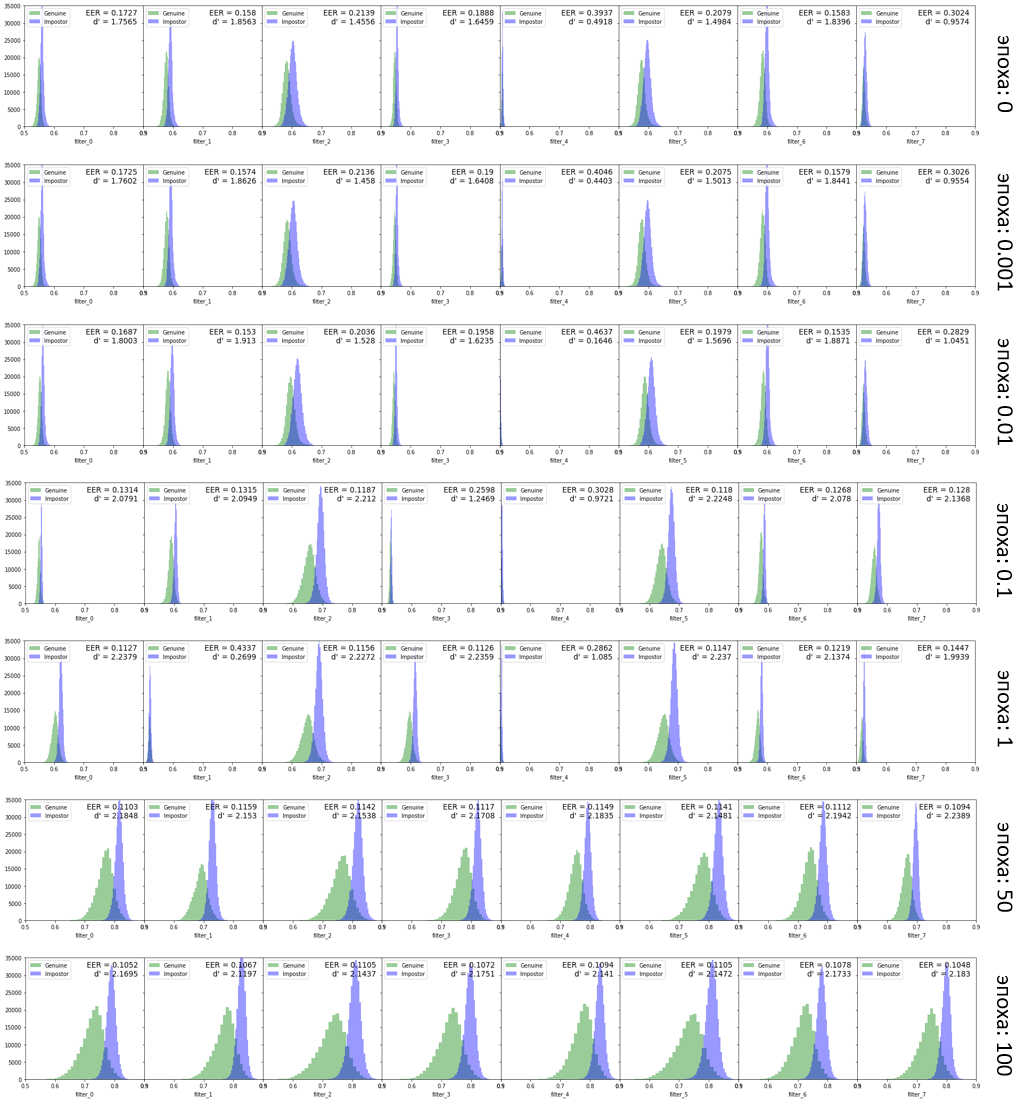
\includegraphics[width=.95\linewidth]{pictures/shfv-distributions-combined.png}
	\end{center}
	\caption{Изменение распределений значений элементов вектора $FV_{sh}$ в процессе обучения}
	\label{fig:shfv-distributions-combined}
\end{figure}

\begin{figure}[h]
	\begin{center}
		
\includegraphics[width=.95\linewidth]{pictures/shfv-filters-100-epoch.png}
	\end{center}
	\caption{Фильтры первого сверточного слоя, полученные после обучения (100 эпох)}
	\label{fig:shfv-filters-100-epoch}
\end{figure}

\begin{figure}[!h]
	\begin{subfigure}{.5\textwidth}
		\centering
		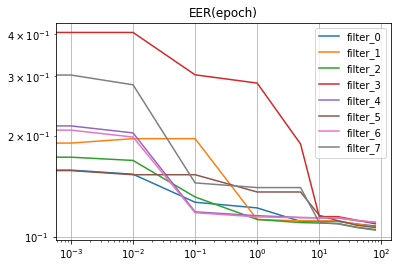
\includegraphics[width=0.95\columnwidth]{pictures/eer_epochs.png}
		\caption{}
		\label{fig:eer_epochs}
	\end{subfigure}%
	\begin{subfigure}{.5\textwidth}
		\centering
		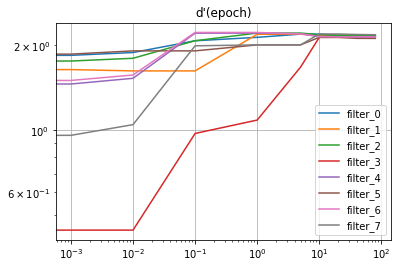
\includegraphics[width=0.95\columnwidth]{pictures/dprime_epochs.png}
		\caption{}
		\label{fig:dprime_epochs}
	\end{subfigure}%
	\caption{Изменение значений EER (а) и d' (б) для распределений элементов вектора $FV_{sh}$ в процессе обучения}
	\label{fig:eer_dprime_epochs}
\end{figure}

\subsection{Высокоуровневое представление признаков}
\label{sec:fem-nn-deepfv}

Представление высокоуровневых (глубоких) признаков выполняется сверточным блоком \#2. Карты признаков $FM^{Sq}_{1,i}$ и $FM^{Sq}_{2,i}$, поступающие из сверточного блока \#1, объединяются по каналам и поступают на вход блоку \#2 (Рис.~\ref{fig:block-scheme-matcher}). Смысл конкатенации на данном этапе  заключается в очередном использовании свойства инвариантности нормализованного изображения радужки. Эксперименты показали преимущества этого подхода по сравнению со стандартными методами~\cite{koch_2015}, где векторы признаков имеют сильно пониженную размерность. Однако среди недостатков такого подхода: относительно большой размер вектора и вычислительная сложность процедуры сравнения. Структура блока представлена в Таб.~\ref{tab:conv-block-2}. Выходной вектор $FV_{deep}\in R^{128} $ отражает высокоуровневое представление отличительных признаков и необходим для работы со сложными нелинейными искажениями текстуры радужной оболочки, вызванными изменением условий окружения.

\begin{table}
	\begin{center}
		\begin{tabular}{|c|c|}
			\hline
			\textbf{Слой}										& \textbf{Размер входного тензора} \\
			\hline
			Сверточный блок $CNNB_{MN} (k_h=k_w=3,s'=2)$ 	& $32\times23\times79$\\
			Сверточный блок $CNNB_{MN} (k_h=k_w=3,s'=2)$ 	& $32\times11\times39$\\
			Сверточный блок $CNNB_{MN} (k_h=k_w=3,s'=1)$ 	& $32\times5\times19$\\
			Полносвязный слой + Пакетная норм. (без акт.)	& $1\times1632$\\
			\hline
		\end{tabular}
		\caption{Структура сверточного блока \#2}
		\label{tab:conv-block-2}
	\end{center}
\end{table}

%-------------------------------------------------------------------------
\subsection{Вычисление степени схожести}

Предварительный анализ ошибок распознавания показал, что genuine и impostor распределения хорошо разделяются. Однако, среди impostor сравнений существуют такие, для которых степень схожести принимает высокие значения, препятствуя фиксированию порога принятия решения на уровне, необходимом для создания устойчивой системы распознавания. Характер распределений элементов $FV_{sh}$ (Рис.~\ref{fig:shfv-distributions-combined}) наталкивает на идею использования методов вариационного вывода для регуляризации. Смысл метода заключается в представлении некоторого вектора в виде $n$-мерной случайной величины с заданным  распределением. В данной работе предлагается представление векторов $FV_{sh}$ и $FV_{deep}$ в виде случайных величин соответствующей размерности, имеющих многомерное нормальное распределение $FV'_{sh}\sim N(\mu_{sh},\Sigma_{sh})$ и $FV'_{deep}\sim N(\mu_{deep},\Sigma_{deep})$ соответственно, где $\mu$ - вектор средних значений, а $\Sigma$ - матрица ковариации. Вариационный вывод в нейронных сетях выполняется при помощи так называемого трюка с переопределением параметров (репараметризацией), описанного в~\cite{kingma_2015}. Выбор (семплирование) значений из распределений выполняется случайным образом и только только в процессе обучения, тогда как для обученной модели выводятся только значения $\mu$. В качества функции активации здесь предлагается использование сигмоида. Эта же процедура выполняется далее для векторов после конкатенации $ FV'_{sh}$, $FV'_{deep}$ и $FV_{add} $, где $FV_{add}=\left\lbrace{\Delta{NPR},AOI}\right\rbrace$, где $AOI$ - площадь пересечения (полезая площадь):

\begin{equation}
\label{eq:aoi}
AOI=\frac{\Sigma{M_c}}{M^h_c\times M^w_c}
\end{equation}

и $\Delta{NPR}$ вычисляется как:

\begin{equation}
\label{eq:dnpr}
\Delta{NPR}=\left|\frac{R^p_1}{R^i_1}-\frac{R^p_2}{R^i_2}\right|
\end{equation}

где $R^p$ и $R^i$ соответствующие радиусы зрачка и радужки

Выходной вектор $FV'_d\in R^{128}$ является входом для последнего полносвязного слоя с двумя нейронами, представляющими два класса: свой и чужой (genuine и impostor). Для Вычисления степени схожести используется \textit{SoftMax} классификатор.

Полученные результаты (Таб.~\ref{tab:exp-results-extreme}) демонстрируют, что применение вариационного вывода (VI) повышает точность распознавания (VI=N означает замену структуры VI на простыми полносвязными слоями соответствующей размерности), но также стоит упомянуть, с увеличением объема данных для обучения, рентабельность применения такого подхода снижается.


%-------------------------------------------------------------------------
\subsection{Метод обучения}

Еще одной особенностью предложенного метода является использование функции потерь (loss function) специального вида. Основная идея заключается в том, что некоторые изображения одной и той же радужки настолько отличаются друг от друга, что их практически невозможно отнести их к одному классу даже визуально по исходному (до нормализации) изображению. Данное свойства в значительной степени препятствует сходимости модели при обучении. Поэтому разумно взвешивать или даже полностью игнорировать такие сравнения при обучении. Предлагается следующий алгоритм:

\begin{enumerate}
	\item[$\bullet$] вычисление функции потерь (например, кросс-энтропии) для каждого сравнения в пакете;
	\item[$\bullet$] применение весов $weights=\lbrace{w_0..w_K}\rbrace$ для $K$-максимальных значений;
	\item[$\bullet$] суммирование значений и вывод значения для пакета;
\end{enumerate}

Данный подход позволил обеспечить лучшую сходимость модели и добиться более высокой точности распознавания.

%-------------------------------------------------------------------------
{\bf Экспериментальные результаты}
\label{sec:fem-nn-exp-results}

Экспериментальные результаты были получены на нескольких наборах данных и сравнивались с наиболее релевантными методами среди существующих. Результаты включают оценку точности распознавания и скорости.

{\bf Экспериментальные данные}
\label{sec:fem-nn-exp-data}

Для обучения и тестирования использовались три разных набора данных: CASIA-Iris-M1-S2 (CMS2)~\cite{casia_mobile_v1}, CASIA-Iris-M1-S3 (CMS3)~\cite{casia_mobile_v1} и еще один (Iris- Mobile, IM), собранный в лаборатории при помощи мобильного устройства со встроенной камерой, работающей в БИК диапазоне. Последний собран, имитируя реальные сценарии аутентификации пользователя мобильного устройства: изображения, захваченные в сильно меняющемся освещении как в помещении, так и на открытом воздухе (под прямым солнечным светом), с очками и без очков. В нем также представлены изображения для людей различных расовых принадлежностей: азиатов и европеоидов. Более подробные спецификации наборов данных описаны в Таб.~\ref{tab:db-description-matcher}, а несколько примеров изображений области глаза представлены на Рис.~\ref{fig:iris-mobile-img-examples}. Выделение области радужки с целью получения масок было осуществлено автоматически алгоритмом, описанным в гл.~\ref{chapter:segmentation}. Примеры изображений радужек и соответствующих масок представлены на Рис.~\ref{fig:block-scheme-matcher}. Каждый набор данных первоначально был разделен на подвыборки: обучающую, валидационную и тестовую в пропорции 70/10/20 (\%) соответственно. Разделение производилось таким образом, что для разных подвыборок не существует изображений одной и той же радужки.

\begin{table}
	\begin{center}
		\begin{tabular}{|c|c|c|c|c|}
			\hline
			\textbf{Набор}	&\textbf{Изображений}	&\textbf{Радужек}	&\textbf{Изображений}	&\textbf{Субъекты}\\
			\textbf{данных}	&\textbf{(всего)}		&\textbf{(всего)}	&\textbf{(на улице)}	&\textbf{}\\
			\hline
			CMS2	&7723	&398	&0			&Азиаты\\
			CMS3	&8167	&720	&0			&Азиаты\\
			IM		&22966	&750	&4933		&Европ. и Азиаты\\
			\hline
		\end{tabular}
		\caption{Описание базы данных тестирования}
		\label{tab:db-description-matcher}
	\end{center}
\end{table}

{\bf Обучение}
\label{sec:fem-nn-training}

Обучение и тестирование проводились отдельно для каждого набора данных. Поскольку количество genuine сравнений $N_G$ намного меньше, все они были использованы для обучения, а количество сравнений impostor было установлено в $N_I=10N_G$. Модель, продемонстрировавшая лучшие результаты на валидационной выборке, выбиралась для оценки на тестовой. Все модели обучались на протяжении 150 эпох, а в качестве метода оптимизации был выбран Adam~\cite{kingma_2014}.

Обучение предлагаемой модели проводилось таким образом, чтобы одна эпоха была эквивалентна одному проходу по всем genuine сравнениям, тогда как impostor сравнения каждый раз случайным образом выбирались из всего набора для каждого пакета. Также была установлена пропорция для количества genuine и impostor сравнений в пакете $N^b_I=10N^b_G$.

{\bf Результаты по точности распознавания}
\label{sec:fem-nn-exp-results-acc}

Полученные результаты по точности распознавания представлены в Таб.~\ref{tab:exp-results-comp} и Рис.~\ref{fig:roc-curves}. Предложенный метод превосходит остальные на всех наборах данных. После разделения полных наборов на подмножества стало невозможно оценить FNMR для FMR=$10^{-7}$ для наборов данных CMS2 и CMS3, поскольку количество сравнений в тестовых подмножествах не превышало 10 миллионов. По этой причине был проведен еще дополнительный эксперимент. Его суть заключалась в том, чтобы оценить эффективность предлагаемой модели на наборах данных без какого-либо обучения или дообучения на них (с переносом). Модель, прошедшая обучение на обучающей выборке IM, была протестирована на полных наборах данных (до разделения) CMS2 и CMS3, чтобы получить FNMR при FMR=$10^{-7}$. Модель показала результаты, превосходящей её собственные, полученные после обучения на обучающих подмножествах данных каждого из наборов, и это доказало её высокую способность к обобщению. Тем не менее, было бы справедливо отметить, что набор данных IM содержит гораздо больше изображений, чем два других.

\begin{table}
	\begin{center}
		\begin{tabular}{|c|c|c|c|}
			\hline
			\textbf{$conv1~|~VI~|~FV_{sh}$}			& \textbf{EER} 		& \textbf{FNMR}		& \textbf{d'} \\
			\hline
			$8\times3\times3~|~Y~|~Y$				& 0.0116	& 0.1925	& 4.3155\\
			$8\times3\times3~|~N~|~Y$				& 0.0120	& 0.2027	& 4.2048\\
			$8\times3\times3~|~Y~|~N$				& 0.0125	& 0.2085	& 4.1253\\
			$8\times9\times9~|~Y~|~Y$				& 0.0134	& 0.1566	& 4.3034\\
			$8\times9\times9~|~Y~|~N$				& 0.0172	& 0.1694	& 3.9850\\
			\hline
		\end{tabular}
		\caption{Оценка точности распознавания для различных модификаций модели}
		\label{tab:exp-results-extreme}
	\end{center}
\end{table}

\begin{table}
	\begin{center}
		\begin{tabular}{|c|c|c|c|c|}
			\hline
			Метод							&CMS2		&CMS3		&IM				&Testing		\\
			\hline
			DeepIrisNet						&0.0709		&0.1199		&0.1371			&без переноса  		\\
			FCN+ETL							&0.0093		&0.0301		&0.0607			&без переноса		\\
			Предложенный					&0.0014		&0.0190		&0.0116			&без переноса		\\
			метод							&0.0003		&0.0086		&0.0116			&с переносом		\\\hline
		\end{tabular}
		\caption{Значения EER, полученные для сравниваемых методов на различных базах данных}
		\label{tab:exp-results-comp}
	\end{center}
\end{table}

\begin{figure}[!h]
	\begin{subfigure}{.33\textwidth}
		\centering
		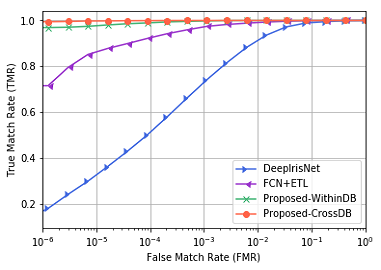
\includegraphics[width=\columnwidth]{pictures/roc-s2.png}
		\caption{}
		\label{fig:roc-s2}
	\end{subfigure}%
	\begin{subfigure}{.33\textwidth}
		\centering
		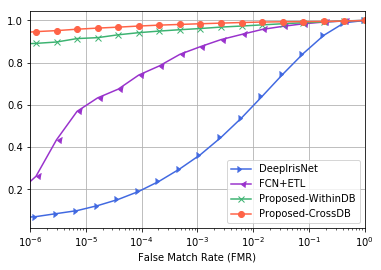
\includegraphics[width=\columnwidth]{pictures/roc-s3.png}
		\caption{}
		\label{fig:roc-s3epochs}
	\end{subfigure}%
	\begin{subfigure}{.33\textwidth}
		\centering
		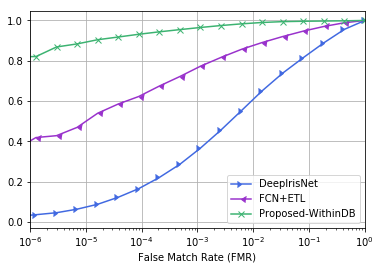
\includegraphics[width=\columnwidth]{pictures/roc-extreme.png}
		\caption{}
		\label{fig:roc-extreme}
	\end{subfigure}%
	\caption{ROC-кривые построенные по результатам тестирования сравниваемых методов на базах данных: (а)CMS2, (б)CMS3, (в)IM}
	\label{fig:roc-curves}
\end{figure}

{\bf Результаты по скорости обработки}
\label{sec:fem-nn-exp-results-speed}

Тестирование предложенного метода производилось на мобильном устройстве. Полное медианное время выполнения измерено на процессоре Qualcomm Snapdragon 835 CPU (2.45 GHz) и составило 3-4 миллисекунды: 1-2 (мсек) для извлечения особенностей и столько же для из сравнения. Измерения производились на одном ядре процессора.

\section{Выводы к четвертой главе}
\label{sec:conclusion-4}

Рассмотрены особенности извлечения и сравнения уникальных особенностей радужки при распознавании в сложных условиях, с учетом специфики применения в мобильном устройстве. Рассмотрены два основных направления к задаче: использование вейвлетов и их всевозможных модификаций, а также методов глубокого обучения. Предложены, протестированы и внедрены два разных метода: (i) основанный на применений вейвлетов Габора с последующим адаптивным квантованием фазы, позволивший достичь большей устойчивости к искажениям текстуры радужки по сравнению с существующими методами; (ii) основанный на применении глубокого обучения с учетом специфики вариативности радужки. Исследована рентабельность использования низкоуровневых текстурных особенностей радужки в объединении с высокоуровневым представлением. В рамках подхода, основанного на применении сверточной нейронной сети предложен новый метод обучения, позволивший обеспечить лучшую сходимость модели и повысить точность распознавания. Для тестирования метода была собрана и подготовлена дополнительная база данных изображений радужек, учитывающая особенности использования мобильного устройства. Оба предложенных метода позволяют обеспечивать высокую скорость распознавания, достаточную для их применения в мобильном устройстве в режиме реального времени.